\chapter{EXPERIMENTAL IMPLEMENTATION}
To complement the numerical findings based on our theoretical framework. We take an experimental implementation to assess two schemes proposed in this work.
The RSSI signal strength data set is collected during experiment. This information is also used to provide statistical evidence for the wireless channel model adopted
throughout. This model is used to determine the characteristics of the environment. The system is designed to work on the 2.4 $GHz$ ISM radio band which is used by Wi-Fi technology. In this experiment, all wireless clients are connected to a wireless access point.
This chapter details the way the experiments are designed, and explains the
analysis of the gathered information.

\section{Monitoring Devices}
Every sensing device takes the form of a Next Unit of Computing (NUC) by Intel{\texttrademark}, and runs on Ubuntu 14.04 operation system. Wireless monitoring is enabled through an Alfa{\texttrademark}~\texttt{AWUS036NHA} wireless interface with a detachable antenna.
The Atheros{\texttrademark} chipset is able to listen to transmission packets on a channel if turned on monitoring mode. The sub-miniature version A antenna connectors are used to attach either isotropic antennas or directional antennas. Each monitoring device is attached with one directional antenna and one isotropic antenna. Wooden sticks are also used to fix the two antennas attached to one monitoring devices at different heights in order to reduce the interference influence between two antennas. The radiation pattern of directional antenna is shown in Fig. \ref{figure:Directionalantenna}.
\begin{figure}[t]
	\centerline{\begin{tikzpicture}
\begin{polaraxis}[
%scale only axis,
width=7cm,
xticklabel=$\pgfmathprintnumber{\tick}^\circ$,
y coord trafo/.code=\pgfmathparse{#1+24},
ytick={-20, -12, 0},
ymin=-25, ymax=4,
y coord inv trafo/.code=\pgfmathparse{#1-24},
%height=5cm,
%xlabel={Angle (degree)},
%ylabel={Gain (dB)},
every tick label/.append style={font=\small},
legend entries={\scriptsize{Directional},
},
legend style={at={(-0.1,0.15)}, nodes=right}
]

% Isotropic
\addplot [
color=black,
densely dotted,
line width=1.5pt
]
coordinates{
(-180,-13.4414512682882)
(-179,-13.4546700300579)
(-178,-13.4764252161895)
(-177,-13.5066749182237)
(-176,-13.5454091452149)
(-175,-13.5926512614262)
(-174,-13.6484593103953)
(-173,-13.7129271845231)
(-172,-13.786185598773)
(-171,-13.8684028282442)
(-170,-13.9597851720984)
(-169,-14.0605771102312)
(-168,-14.171061123622)
(-167,-14.2915571537574)
(-166,-14.4224216799846)
(-165,-14.564046395037)
(-164,-14.7168564570345)
(-163,-14.8813082895423)
(-162,-15.0578868880923)
(-161,-15.2471025699203)
(-160,-15.4494870710865)
(-159,-15.6655888485296)
(-158,-15.8959673799491)
(-157,-16.1411861664687)
(-156,-16.4018040249311)
(-155,-16.6783640994064)
(-154,-16.9713798135067)
(-153,-17.2813167120243)
(-152,-17.6085687852638)
(-151,-17.9534274140926)
(-150,-18.3160405027914)
(-149,-18.6963586762959)
(-148,-19.0940646335486)
(-147,-19.5084809568845)
(-146,-19.9384510871974)
(-145,-20.3821882119969)
(-144,-20.8370882639926)
(-143,-21.2995074098521)
(-142,-21.7645132926185)
(-141,-22.225635323862)
(-140,-22.6746644506975)
(-139,-23.1015859631804)
(-138,-23.4947613901067)
(-137,-23.841486082104)
(-136,-24.1290045299321)
(-135,-24.345937785169)
(-134,-24.4838807689049)
(-133,-24.538750169525)
(-132,-24.5114404842924)
(-131,-24.4075490242601)
(-130,-24.2362736547105)
(-129,-24.0088681874837)
(-128,-23.7371101123833)
(-127,-23.4321061663679)
(-126,-23.1035576892841)
(-125,-22.7594458246612)
(-124,-22.4060195668596)
(-123,-22.0479616840587)
(-122,-21.6886342872691)
(-121,-21.3303403105187)
(-120,-20.9745660215661)
(-119,-20.6221893280437)
(-118,-20.2736501988418)
(-117,-19.9290854147959)
(-116,-19.5884323141828)
(-115,-19.2515067852031)
(-114,-18.918060457562)
(-113,-18.5878214048584)
(-112,-18.2605219640107)
(-111,-17.9359166277138)
(-110,-17.6137924101798)
(-109,-17.29397362645)
(-108,-16.976322648047)
(-107,-16.6607378863736)
(-106,-16.3471499957831)
(-105,-16.035517069923)
(-104,-15.7258194204318)
(-103,-15.4180543715238)
(-102,-15.1122313742234)
(-101,-14.8083676376039)
(-100,-14.506484389242)
(-99,-14.2066038110712)
(-98,-13.9087466476471)
(-97,-13.6129304491279)
(-96,-13.3191683886201)
(-95,-13.0274685805737)
(-94,-12.7378338214717)
(-93,-12.4502616741834)
(-92,-12.1647448213794)
(-91,-11.8812716199649)
(-90,-11.5998267964784)
(-89,-11.3203922319979)
(-88,-11.0429477936784)
(-87,-10.7674721782015)
(-86,-10.4939437398711)
(-85,-10.2223412826925)
(-84,-9.95264480145817)
(-83,-9.68483616163374)
(-82,-9.41889971173306)
(-81,-9.15482282496653)
(-80,-8.89259636932495)
(-79,-8.63221510702225)
(-78,-8.37367802545644)
(-77,-8.11698860265535)
(-76,-7.86215501063776)
(-75,-7.60919026032084)
(-74,-7.35811229161282)
(-73,-7.10894401220511)
(-72,-6.86171328837428)
(-71,-6.61645289086147)
(-70,-6.37320039865155)
(-69,-6.13199806324974)
(-68,-5.89289263586871)
(-67,-5.65593515980614)
(-66,-5.42118073021528)
(-65,-5.18868822345142)
(-64,-4.95851999820981)
(-63,-4.73074157075047)
(-62,-4.50542126662129)
(-61,-4.2826298514338)
(-60,-4.06244014340366)
(-59,-3.84492661052946)
(-58,-3.63016495543777)
(-57,-3.41823169106094)
(-56,-3.20920371042792)
(-55,-3.00315785393204)
(-54,-2.80017047748882)
(-53,-2.60031702500869)
(-52,-2.40367160858357)
(-51,-2.21030659972392)
(-50,-2.02029223488485)
(-49,-1.83369623839114)
(-48,-1.65058346571357)
(-47,-1.47101556986747)
(-46,-1.29505069350371)
(-45,-1.12274318904406)
(-44,-0.954143368983411)
(-43,-0.789297288240012)
(-42,-0.628246560187275)
(-41,-0.471028207745463)
(-40,-0.3176745506513)
(-39,-0.168213129757901)
(-38,-0.0226666689462413)
(-37,0.118946925047271)
(-36,0.2566145248653)
(-35,0.390327707093715)
(-34,0.52008263971821)
(-33,0.64587993333766)
(-32,0.767724457304659)
(-31,0.885625122272774)
(-30,0.999594630939741)
(-29,1.10964919908268)
(-28,1.2158082492813)
(-27,1.31809408001364)
(-26,1.41653151308021)
(-25,1.51114752256122)
(-24,1.6019708487323)
(-23,1.68903160054985)
(-22,1.77236085046353)
(-21,1.85199022541475)
(-20,1.9279514979322)
(-19,2.00027618123524)
(-18,2.06899513220245)
(-17,2.13413816595322)
(-16,2.19573368562859)
(-15,2.25380833074432)
(-14,2.30838664722957)
(-13,2.35949078196381)
(-12,2.40714020429038)
(-11,2.45135145662405)
(-10,2.4921379358927)
(-9,2.52950970716712)
(-8,2.56347335044864)
(-7,2.59403184120972)
(-6,2.62118446492706)
(-5,2.64492676551581)
(-4,2.66525052727538)
(-3,2.6821437896941)
(-2,2.6955908942363)
(-1,2.70557256205164)
(0,2.71206600140163)
(1,2.71504504349215)
(2,2.71448030532699)
(3,2.71033937815481)
(4,2.70258704006228)
(5,2.69118549126542)
(6,2.67609461066265)
(7,2.65727223223051)
(8,2.63467443986141)
(9,2.6082558792568)
(10,2.57797008549462)
(11,2.54376982488378)
(12,2.50560744969799)
(13,2.46343526434591)
(14,2.41720590148354)
(15,2.36687270650855)
(16,2.3123901287964)
(17,2.25371411794659)
(18,2.19080252320585)
(19,2.12361549412707)
(20,2.05211588040985)
(21,1.97626962875452)
(22,1.89604617444716)
(23,1.81141882528301)
(24,1.72236513532894)
(25,1.99175117988582)
(26,1.53091233124645)
(27,1.42849272561821)
(29,1.21025729324901)
(30,1.09445528952659)
(31,0.974216741709544)
(32,0.849564514944864)
(33,0.720528173063555)
(34,0.587144096307417)
(35,0.449455557245233)
(36,0.307512752045061)
(37,0.161372784395877)
(38,0.0110995995431912)
(39,-0.143236133871139)
(40,-0.301557196188855)
(41,-0.463780045003785)
(42,-0.62981510055741)
(43,-0.799567088987819)
(44,-0.972935443560481)
(45,-1.1498147633239)
(46,-1.33009532786158)
(47,-1.51366366595923)
(48,-1.70040317508237)
(49,-1.89019478757868)
(50,-2.08291767850118)
(51,-2.27845000891792)
(52,-2.47666969755972)
(53,-2.67745521269372)
(54,-2.88068637523409)
(55,-3.08624516334933)
(56,-3.29401650823699)
(57,-3.50388907034674)
(58,-3.71575598517274)
(59,-3.9295155678316)
(60,-4.14507196600797)
(61,-4.36233575149249)
(62,-4.58122444145012)
(63,-4.80166294172245)
(64,-5.023583905855)
(65,-5.24692800510786)
(66,-5.47164410640298)
(67,-5.69768935692525)
(68,-5.92502917586247)
(69,-6.15363715547638)
(70,-6.38349487527737)
(71,-6.61459163447289)
(72,-6.84692410902017)
(73,-7.08049594049927)
(74,-7.31531726460218)
(75,-7.55140418729642)
(76,-7.7887782166628)
(77,-8.02746565804477)
(78,-8.26749697950575)
(79,-8.50890615371232)
(80,-8.7517299812968)
(81,-8.99600739956453)
(82,-9.24177877916908)
(83,-9.48908521016268)
(84,-9.73796777772268)
(85,-9.98846682695023)
(86,-10.2406212155298)
(87,-10.4944675528249)
(88,-10.7500394242691)
(89,-11.0073666007915)
(90,-11.2664742345827)
(91,-11.527382044853)
(92,-11.7901035004158)
(93,-12.0546450099917)
(94,-12.3210051360608)
(95,-12.5891738538252)
(96,-12.8591318832415)
(97,-13.1308501288662)
(98,-13.4042892690602)
(99,-13.6793995423239)
(100,-13.9561207834602)
(101,-14.2343827648686)
(102-14.5141058973709)
(103,-14.7952023390768)
(104,-15.0775775482592)
(105,-15.3611322951881)
(106,-15.6457651164751)
(107,-15.931375151856)
(108,-16.2178652458555)
(109,-16.5051451241594)
(110,-16.7931343660336)
(111,-17.0817647896647)
(112,-17.3709817474832)
(113,-17.660743694628)
(114,-17.9510192476875)
(115,-18.2417807953044)
(116,-18.5329935608064)
(117,-18.8245988554148)
(118,-19.1164901088089)
(119,-19.4084801405945)
(120,-19.7002580763119)
(121,-19.9913343773253)
(122,-20.2809727512362)
(123,-20.568108407892)
(124,-20.8512534776172)
(125,-21.1283927526256)
(126,-21.3968766416795)
(127,-21.6533236640386)
(128,-21.8935519309185)
(129,-22.1125670348475)
(130,-22.3046403175387)
(131,-22.4635124516099)
(132,-22.5827470152761)
(133,-22.6562324006537)
(134,-22.6787882718734)
(135,-22.6467850057595)
(136,-22.5586514104813)
(137,-22.4151496027575)
(138,-22.2193449738644)
(139,-21.9762785037077)
(140,-21.6924248400978)
(141,-21.3750610806376)
(142,-21.0316671990914)
(143,-20.6694416923696)
(144,-20.2949680530151)
(145,-19.9140279528015)
(146,-19.5315337437566)
(147,-19.1515450608419)
(148,-18.7773366811067)
(149,-18.4114918745034)
(150,-18.0560034400361)
(151,-17.7123714767822)
(152,-17.3816920394535)
(153,-17.0647342403978)
(154,-16.762005436053)
(155,-16.4738052695645)
(156,-16.2002698648214)
(157,-15.9414076250108)
(158,-15.6971280456792)
(159,-15.4672648118864)
(160,-15.2515942726462)
(161,-15.0498502072073)
(162,-14.8617356336503)
(163,-14.6869322676632)
(164,-14.5251081196561)
(165,-14.375923620256)
(166,-14.2390365851378)
(167,-14.1141062671784)
(168,-14.0007966942181)
(169,-13.8987794517061)
(170,-13.8077360389446)
(171,-13.7273599036436)
(172,-13.6573582404617)
(173,-13.5974536238536)
(174,-13.5473855327981)
(175,-13.50691181402)
(176,-13.4758101204807)
(177,-13.4538793527298)
(178,-13.4409411218528)
(179,-13.4368412440497)
(180,-13.4414512682882)

};

% Theta3dB = 60.0
\addplot [
color=white,
dashed,
line width=1.0pt
]
coordinates{
(-180, -12.6128) (-179, -12.6128) (-178, -12.6128) (-177, -12.6128)
(-176, -12.6128) (-175, -12.6128) (-174, -12.6128) (-173, -12.6128)
(-172, -12.6128) (-171, -12.6128) (-170, -12.6128) (-169, -12.6128)
(-168, -12.6128) (-167, -12.6128) (-166, -12.6128) (-165, -12.6128)
(-164, -12.6128) (-163, -12.6128) (-162, -12.6128) (-161, -12.6128)
(-160, -12.6128) (-159, -12.6128) (-158, -12.6128) (-157, -12.6128)
(-156, -12.6128) (-155, -12.6128) (-154, -12.6128) (-153, -12.6128)
(-152, -12.6128) (-151, -12.6128) (-150, -12.6128) (-149, -12.6128)
(-148, -12.6128) (-147, -12.6128) (-146, -12.6128) (-145, -12.6128)
(-144, -12.6128) (-143, -12.6128) (-142, -12.6128) (-141, -12.6128)
(-140, -12.6128) (-139, -12.6128) (-138, -12.6128) (-137, -12.6128)
(-136, -12.6128) (-135, -12.6128) (-134, -12.6128) (-133, -12.6128)
(-132, -12.6128) (-131, -12.6128) (-130, -12.6128) (-129, -12.6128)
(-128, -12.6128) (-127, -12.6128) (-126, -12.6128) (-125, -12.6128)
(-124, -12.6128) (-123, -12.6128) (-122, -12.6128) (-121, -12.6128)
(-120, -12.6128) (-119, -12.6128) (-118, -12.6128) (-117, -12.6128)
(-116, -12.6128) (-115, -12.6128) (-114, -12.6128) (-113, -12.6128)
(-112, -12.6128) (-111, -12.6128) (-110, -12.6128) (-109, -12.6128)
(-108, -12.6128) (-107, -12.6128) (-106, -12.6128) (-105, -12.6128)
(-104, -12.6128) (-103, -12.6128) (-102, -12.6128) (-101, -12.6128)
(-100, -12.6128) (-99, -12.6128) (-98, -12.6128) (-97, -12.6128)
(-96, -12.6128) (-95, -12.6128) (-94, -12.6128) (-93, -12.6128)
(-92, -12.6128) (-91, -12.6128) (-90, -12.6128) (-89, -12.6128)
(-88, -12.6128) (-87, -12.6128) (-86, -12.6128) (-85, -12.6128)
(-84, -12.6128) (-83, -12.6128) (-82, -12.6128) (-81, -12.6128)
(-80, -12.6128) (-79, -12.6128) (-78, -12.6128) (-77, -12.3761)
(-76, -11.8661) (-75, -11.3628) (-74, -10.8661) (-73, -10.3761)
(-72, -9.8928) (-71, -9.4161) (-70, -8.9461) (-69, -8.4828)
(-68, -8.0261) (-67, -7.5761) (-66, -7.1328) (-65, -6.6961)
(-64, -6.2661) (-63, -5.8428) (-62, -5.4261) (-61, -5.0161)
(-60, -4.6128) (-59, -4.2161) (-58, -3.8261) (-57, -3.4428)
(-56, -3.0661) (-55, -2.6961) (-54, -2.3328) (-53, -1.9761)
(-52, -1.6261) (-51, -1.2828) (-50, -0.9461) (-49, -0.6161)
(-48, -0.2928) (-47, 0.0239) (-46, 0.3339) (-45, 0.6372)
(-44, 0.9339) (-43, 1.2239) (-42, 1.5072) (-41, 1.7839)
(-40, 2.0539) (-39, 2.3172) (-38, 2.5739) (-37, 2.8239)
(-36, 3.0672) (-35, 3.3039) (-34, 3.5339) (-33, 3.7572)
(-32, 3.9739) (-31, 4.1839) (-30, 4.3872) (-29, 4.5839)
(-28, 4.7739) (-27, 4.9572) (-26, 5.1339) (-25, 5.3039)
(-24, 5.4672) (-23, 5.6239) (-22, 5.7739) (-21, 5.9172)
(-20, 6.0539) (-19, 6.1839) (-18, 6.3072) (-17, 6.4239)
(-16, 6.5339) (-15, 6.6372) (-14, 6.7339) (-13, 6.8239)
(-12, 6.9072) (-11, 6.9839) (-10, 7.0539) ( -9, 7.1172)
( -8, 7.1739) ( -7, 7.2239) ( -6, 7.2672) ( -5, 7.3039)
( -4, 7.3339) ( -3, 7.3572) ( -2, 7.3739) ( -1, 7.3839)
(  0, 7.3872) (  1, 7.3839) (  2, 7.3739) (  3, 7.3572)
(  4, 7.3339) (  5, 7.3039) (  6, 7.2672) (  7, 7.2239)
(  8, 7.1739) (  9, 7.1172) ( 10, 7.0539) ( 11, 6.9839)
( 12, 6.9072) ( 13, 6.8239) ( 14, 6.7339) ( 15, 6.6372)
( 16, 6.5339) ( 17, 6.4239) ( 18, 6.3072) ( 19, 6.1839)
( 20, 6.0539) ( 21, 5.9172) ( 22, 5.7739) ( 23, 5.6239)
( 24, 5.4672) ( 25, 5.3039) ( 26, 5.1339) ( 27, 4.9572)
( 28, 4.7739) ( 29, 4.5839) ( 30, 4.3872) ( 31, 4.1839)
( 32, 3.9739) ( 33, 3.7572) ( 34, 3.5339) ( 35, 3.3039)
( 36, 3.0672) ( 37, 2.8239) ( 38, 2.5739) ( 39, 2.3172)
( 40, 2.0539) ( 41, 1.7839) ( 42, 1.5072) ( 43, 1.2239)
( 44, 0.9339) ( 45, 0.6372) ( 46, 0.3339) ( 47, 0.0239)
( 48, -0.2928) ( 49, -0.6161) ( 50, -0.9461) ( 51, -1.2828)
( 52, -1.6261) ( 53, -1.9761) ( 54, -2.3328) ( 55, -2.6961)
( 56, -3.0661) ( 57, -3.4428) ( 58, -3.8261) ( 59, -4.2161)
( 60, -4.6128) ( 61, -5.0161) ( 62, -5.4261) ( 63, -5.8428)
( 64, -6.2661) ( 65, -6.6961) ( 66, -7.1328) ( 67, -7.5761)
( 68, -8.0261) ( 69, -8.4828) ( 70, -8.9461) ( 71, -9.4161)
( 72, -9.8928) ( 73, -10.3761) ( 74, -10.8661) ( 75, -11.3628)
( 76, -11.8661) ( 77, -12.3761) ( 78, -12.6128) ( 79, -12.6128)
( 80, -12.6128) ( 81, -12.6128) ( 82, -12.6128) ( 83, -12.6128)
( 84, -12.6128) ( 85, -12.6128) ( 86, -12.6128) ( 87, -12.6128)
( 88, -12.6128) ( 89, -12.6128) ( 90, -12.6128) ( 91, -12.6128)
( 92, -12.6128) ( 93, -12.6128) ( 94, -12.6128) ( 95, -12.6128)
( 96, -12.6128) ( 97, -12.6128) ( 98, -12.6128) ( 99, -12.6128)
(100, -12.6128) (101, -12.6128) (102, -12.6128) (103, -12.6128)
(104, -12.6128) (105, -12.6128) (106, -12.6128) (107, -12.6128)
(108, -12.6128) (109, -12.6128) (110, -12.6128) (111, -12.6128)
(112, -12.6128) (113, -12.6128) (114, -12.6128) (115, -12.6128)
(116, -12.6128) (117, -12.6128) (118, -12.6128) (119, -12.6128)
(120, -12.6128) (121, -12.6128) (122, -12.6128) (123, -12.6128)
(124, -12.6128) (125, -12.6128) (126, -12.6128) (127, -12.6128)
(128, -12.6128) (129, -12.6128) (130, -12.6128) (131, -12.6128)
(132, -12.6128) (133, -12.6128) (134, -12.6128) (135, -12.6128)
(136, -12.6128) (137, -12.6128) (138, -12.6128) (139, -12.6128)
(140, -12.6128) (141, -12.6128) (142, -12.6128) (143, -12.6128)
(144, -12.6128) (145, -12.6128) (146, -12.6128) (147, -12.6128)
(148, -12.6128) (149, -12.6128) (150, -12.6128) (151, -12.6128)
(152, -12.6128) (153, -12.6128) (154, -12.6128) (155, -12.6128)
(156, -12.6128) (157, -12.6128) (158, -12.6128) (159, -12.6128)
(160, -12.6128) (161, -12.6128) (162, -12.6128) (163, -12.6128)
(164, -12.6128) (165, -12.6128) (166, -12.6128) (167, -12.6128)
(168, -12.6128) (169, -12.6128) (170, -12.6128) (171, -12.6128)
(172, -12.6128) (173, -12.6128) (174, -12.6128) (175, -12.6128)
(176, -12.6128) (177, -12.6128) (178, -12.6128) (179, -12.6128)
(180, -12.6128)
};

% Theta3dB = 90.0
\addplot [
color=white,
solid,
line width=1.5pt
]
coordinates{
(-180, -14.2936) (-179, -14.2936) (-178, -14.2936) (-177, -14.2936)
(-176, -14.2936) (-175, -14.2936) (-174, -14.2936) (-173, -14.2936)
(-172, -14.2936) (-171, -14.2936) (-170, -14.2936) (-169, -14.2936)
(-168, -14.2936) (-167, -14.2936) (-166, -14.2936) (-165, -14.2936)
(-164, -14.2936) (-163, -14.2936) (-162, -14.2936) (-161, -14.2936)
(-160, -14.2936) (-159, -14.2936) (-158, -14.2936) (-157, -14.2936)
(-156, -14.2936) (-155, -14.2936) (-154, -14.2936) (-153, -14.2936)
(-152, -14.2936) (-151, -14.2936) (-150, -14.2936) (-149, -14.2936)
(-148, -14.2936) (-147, -14.2936) (-146, -14.2936) (-145, -14.2936)
(-144, -14.2936) (-143, -14.2936) (-142, -14.2936) (-141, -14.2936)
(-140, -14.2936) (-139, -14.2936) (-138, -14.2936) (-137, -14.2936)
(-136, -14.2936) (-135, -14.2936) (-134, -14.2936) (-133, -14.2936)
(-132, -14.2936) (-131, -14.2936) (-130, -14.2936) (-129, -14.2936)
(-128, -14.2936) (-127, -14.2936) (-126, -14.2936) (-125, -14.2936)
(-124, -14.2936) (-123, -14.2936) (-122, -14.2936) (-121, -14.2936)
(-120, -14.2936) (-119, -14.2936) (-118, -14.2936) (-117, -14.2936)
(-116, -14.2284) (-115, -13.8862) (-114, -13.5469) (-113, -13.2106)
(-112, -12.8773) (-111, -12.5469) (-110, -12.2195) (-109, -11.8951)
(-108, -11.5736) (-107, -11.2551) (-106, -10.9395) (-105, -10.6269)
(-104, -10.3173) (-103, -10.0106) (-102, -9.7069) (-101, -9.4062)
(-100, -9.1084) (-99, -8.8136) (-98, -8.5218) (-97, -8.2329)
(-96, -7.9469) (-95, -7.6640) (-94, -7.3840) (-93, -7.1069)
(-92, -6.8329) (-91, -6.5618) (-90, -6.2936) (-89, -6.0284)
(-88, -5.7662) (-87, -5.5069) (-86, -5.2506) (-85, -4.9973)
(-84, -4.7469) (-83, -4.4995) (-82, -4.2551) (-81, -4.0136)
(-80, -3.7751) (-79, -3.5395) (-78, -3.3069) (-77, -3.0773)
(-76, -2.8506) (-75, -2.6269) (-74, -2.4062) (-73, -2.1884)
(-72, -1.9736) (-71, -1.7618) (-70, -1.5529) (-69, -1.3469)
(-68, -1.1440) (-67, -0.9440) (-66, -0.7469) (-65, -0.5529)
(-64, -0.3618) (-63, -0.1736) (-62, 0.0116) (-61, 0.1938)
(-60, 0.3731) (-59, 0.5494) (-58, 0.7227) (-57, 0.8931)
(-56, 1.0605) (-55, 1.2249) (-54, 1.3864) (-53, 1.5449)
(-52, 1.7005) (-51, 1.8531) (-50, 2.0027) (-49, 2.1494)
(-48, 2.2931) (-47, 2.4338) (-46, 2.5716) (-45, 2.7064)
(-44, 2.8382) (-43, 2.9671) (-42, 3.0931) (-41, 3.2160)
(-40, 3.3360) (-39, 3.4531) (-38, 3.5671) (-37, 3.6782)
(-36, 3.7864) (-35, 3.8916) (-34, 3.9938) (-33, 4.0931)
(-32, 4.1894) (-31, 4.2827) (-30, 4.3731) (-29, 4.4605)
(-28, 4.5449) (-27, 4.6264) (-26, 4.7049) (-25, 4.7805)
(-24, 4.8531) (-23, 4.9227) (-22, 4.9894) (-21, 5.0531)
(-20, 5.1138) (-19, 5.1716) (-18, 5.2264) (-17, 5.2782)
(-16, 5.3271) (-15, 5.3731) (-14, 5.4160) (-13, 5.4560)
(-12, 5.4931) (-11, 5.5271) (-10, 5.5582) ( -9, 5.5864)
( -8, 5.6116) ( -7, 5.6338) ( -6, 5.6531) ( -5, 5.6694)
( -4, 5.6827) ( -3, 5.6931) ( -2, 5.7005) ( -1, 5.7049)
(  0, 5.7064) (  1, 5.7049) (  2, 5.7005) (  3, 5.6931)
(  4, 5.6827) (  5, 5.6694) (  6, 5.6531) (  7, 5.6338)
(  8, 5.6116) (  9, 5.5864) ( 10, 5.5582) ( 11, 5.5271)
( 12, 5.4931) ( 13, 5.4560) ( 14, 5.4160) ( 15, 5.3731)
( 16, 5.3271) ( 17, 5.2782) ( 18, 5.2264) ( 19, 5.1716)
( 20, 5.1138) ( 21, 5.0531) ( 22, 4.9894) ( 23, 4.9227)
( 24, 4.8531) ( 25, 4.7805) ( 26, 4.7049) ( 27, 4.6264)
( 28, 4.5449) ( 29, 4.4605) ( 30, 4.3731) ( 31, 4.2827)
( 32, 4.1894) ( 33, 4.0931) ( 34, 3.9938) ( 35, 3.8916)
( 36, 3.7864) ( 37, 3.6782) ( 38, 3.5671) ( 39, 3.4531)
( 40, 3.3360) ( 41, 3.2160) ( 42, 3.0931) ( 43, 2.9671)
( 44, 2.8382) ( 45, 2.7064) ( 46, 2.5716) ( 47, 2.4338)
( 48, 2.2931) ( 49, 2.1494) ( 50, 2.0027) ( 51, 1.8531)
( 52, 1.7005) ( 53, 1.5449) ( 54, 1.3864) ( 55, 1.2249)
( 56, 1.0605) ( 57, 0.8931) ( 58, 0.7227) ( 59, 0.5494)
( 60, 0.3731) ( 61, 0.1938) ( 62, 0.0116) ( 63, -0.1736)
( 64, -0.3618) ( 65, -0.5529) ( 66, -0.7469) ( 67, -0.9440)
( 68, -1.1440) ( 69, -1.3469) ( 70, -1.5529) ( 71, -1.7618)
( 72, -1.9736) ( 73, -2.1884) ( 74, -2.4062) ( 75, -2.6269)
( 76, -2.8506) ( 77, -3.0773) ( 78, -3.3069) ( 79, -3.5395)
( 80, -3.7751) ( 81, -4.0136) ( 82, -4.2551) ( 83, -4.4995)
( 84, -4.7469) ( 85, -4.9973) ( 86, -5.2506) ( 87, -5.5069)
( 88, -5.7662) ( 89, -6.0284) ( 90, -6.2936) ( 91, -6.5618)
( 92, -6.8329) ( 93, -7.1069) ( 94, -7.3840) ( 95, -7.6640)
( 96, -7.9469) ( 97, -8.2329) ( 98, -8.5218) ( 99, -8.8136)
(100, -9.1084) (101, -9.4062) (102, -9.7069) (103, -10.0106)
(104, -10.3173) (105, -10.6269) (106, -10.9395) (107, -11.2551)
(108, -11.5736) (109, -11.8951) (110, -12.2195) (111, -12.5469)
(112, -12.8773) (113, -13.2106) (114, -13.5469) (115, -13.8862)
(116, -14.2284) (117, -14.2936) (118, -14.2936) (119, -14.2936)
(120, -14.2936) (121, -14.2936) (122, -14.2936) (123, -14.2936)
(124, -14.2936) (125, -14.2936) (126, -14.2936) (127, -14.2936)
(128, -14.2936) (129, -14.2936) (130, -14.2936) (131, -14.2936)
(132, -14.2936) (133, -14.2936) (134, -14.2936) (135, -14.2936)
(136, -14.2936) (137, -14.2936) (138, -14.2936) (139, -14.2936)
(140, -14.2936) (141, -14.2936) (142, -14.2936) (143, -14.2936)
(144, -14.2936) (145, -14.2936) (146, -14.2936) (147, -14.2936)
(148, -14.2936) (149, -14.2936) (150, -14.2936) (151, -14.2936)
(152, -14.2936) (153, -14.2936) (154, -14.2936) (155, -14.2936)
(156, -14.2936) (157, -14.2936) (158, -14.2936) (159, -14.2936)
(160, -14.2936) (161, -14.2936) (162, -14.2936) (163, -14.2936)
(164, -14.2936) (165, -14.2936) (166, -14.2936) (167, -14.2936)
(168, -14.2936) (169, -14.2936) (170, -14.2936) (171, -14.2936)
(172, -14.2936) (173, -14.2936) (174, -14.2936) (175, -14.2936)
(176, -14.2936) (177, -14.2936) (178, -14.2936) (179, -14.2936)
(180, -14.2936)
};

% Theta3dB = 120.0
\addplot [
color=white,
dashdotted,
line width=1.0pt
]
coordinates{
(-180, -15.5024) (-179, -15.5024) (-178, -15.5024) (-177, -15.5024)
(-176, -15.5024) (-175, -15.5024) (-174, -15.5024) (-173, -15.5024)
(-172, -15.5024) (-171, -15.5024) (-170, -15.5024) (-169, -15.5024)
(-168, -15.5024) (-167, -15.5024) (-166, -15.5024) (-165, -15.5024)
(-164, -15.5024) (-163, -15.5024) (-162, -15.5024) (-161, -15.5024)
(-160, -15.5024) (-159, -15.5024) (-158, -15.5024) (-157, -15.5024)
(-156, -15.5024) (-155, -15.5024) (-154, -15.2657) (-153, -15.0099)
(-152, -14.7557) (-151, -14.5032) (-150, -14.2524) (-149, -14.0032)
(-148, -13.7557) (-147, -13.5099) (-146, -13.2657) (-145, -13.0232)
(-144, -12.7824) (-143, -12.5432) (-142, -12.3057) (-141, -12.0699)
(-140, -11.8357) (-139, -11.6032) (-138, -11.3724) (-137, -11.1432)
(-136, -10.9157) (-135, -10.6899) (-134, -10.4657) (-133, -10.2432)
(-132, -10.0224) (-131, -9.8032) (-130, -9.5857) (-129, -9.3699)
(-128, -9.1557) (-127, -8.9432) (-126, -8.7324) (-125, -8.5232)
(-124, -8.3157) (-123, -8.1099) (-122, -7.9057) (-121, -7.7032)
(-120, -7.5024) (-119, -7.3032) (-118, -7.1057) (-117, -6.9099)
(-116, -6.7157) (-115, -6.5232) (-114, -6.3324) (-113, -6.1432)
(-112, -5.9557) (-111, -5.7699) (-110, -5.5857) (-109, -5.4032)
(-108, -5.2224) (-107, -5.0432) (-106, -4.8657) (-105, -4.6899)
(-104, -4.5157) (-103, -4.3432) (-102, -4.1724) (-101, -4.0032)
(-100, -3.8357) (-99, -3.6699) (-98, -3.5057) (-97, -3.3432)
(-96, -3.1824) (-95, -3.0232) (-94, -2.8657) (-93, -2.7099)
(-92, -2.5557) (-91, -2.4032) (-90, -2.2524) (-89, -2.1032)
(-88, -1.9557) (-87, -1.8099) (-86, -1.6657) (-85, -1.5232)
(-84, -1.3824) (-83, -1.2432) (-82, -1.1057) (-81, -0.9699)
(-80, -0.8357) (-79, -0.7032) (-78, -0.5724) (-77, -0.4432)
(-76, -0.3157) (-75, -0.1899) (-74, -0.0657) (-73, 0.0568)
(-72, 0.1776) (-71, 0.2968) (-70, 0.4143) (-69, 0.5301)
(-68, 0.6443) (-67, 0.7568) (-66, 0.8676) (-65, 0.9768)
(-64, 1.0843) (-63, 1.1901) (-62, 1.2943) (-61, 1.3968)
(-60, 1.4976) (-59, 1.5968) (-58, 1.6943) (-57, 1.7901)
(-56, 1.8843) (-55, 1.9768) (-54, 2.0676) (-53, 2.1568)
(-52, 2.2443) (-51, 2.3301) (-50, 2.4143) (-49, 2.4968)
(-48, 2.5776) (-47, 2.6568) (-46, 2.7343) (-45, 2.8101)
(-44, 2.8843) (-43, 2.9568) (-42, 3.0276) (-41, 3.0968)
(-40, 3.1643) (-39, 3.2301) (-38, 3.2943) (-37, 3.3568)
(-36, 3.4176) (-35, 3.4768) (-34, 3.5343) (-33, 3.5901)
(-32, 3.6443) (-31, 3.6968) (-30, 3.7476) (-29, 3.7968)
(-28, 3.8443) (-27, 3.8901) (-26, 3.9343) (-25, 3.9768)
(-24, 4.0176) (-23, 4.0568) (-22, 4.0943) (-21, 4.1301)
(-20, 4.1643) (-19, 4.1968) (-18, 4.2276) (-17, 4.2568)
(-16, 4.2843) (-15, 4.3101) (-14, 4.3343) (-13, 4.3568)
(-12, 4.3776) (-11, 4.3968) (-10, 4.4143) ( -9, 4.4301)
( -8, 4.4443) ( -7, 4.4568) ( -6, 4.4676) ( -5, 4.4768)
( -4, 4.4843) ( -3, 4.4901) ( -2, 4.4943) ( -1, 4.4968)
(  0, 4.4976) (  1, 4.4968) (  2, 4.4943) (  3, 4.4901)
(  4, 4.4843) (  5, 4.4768) (  6, 4.4676) (  7, 4.4568)
(  8, 4.4443) (  9, 4.4301) ( 10, 4.4143) ( 11, 4.3968)
( 12, 4.3776) ( 13, 4.3568) ( 14, 4.3343) ( 15, 4.3101)
( 16, 4.2843) ( 17, 4.2568) ( 18, 4.2276) ( 19, 4.1968)
( 20, 4.1643) ( 21, 4.1301) ( 22, 4.0943) ( 23, 4.0568)
( 24, 4.0176) ( 25, 3.9768) ( 26, 3.9343) ( 27, 3.8901)
( 28, 3.8443) ( 29, 3.7968) ( 30, 3.7476) ( 31, 3.6968)
( 32, 3.6443) ( 33, 3.5901) ( 34, 3.5343) ( 35, 3.4768)
( 36, 3.4176) ( 37, 3.3568) ( 38, 3.2943) ( 39, 3.2301)
( 40, 3.1643) ( 41, 3.0968) ( 42, 3.0276) ( 43, 2.9568)
( 44, 2.8843) ( 45, 2.8101) ( 46, 2.7343) ( 47, 2.6568)
( 48, 2.5776) ( 49, 2.4968) ( 50, 2.4143) ( 51, 2.3301)
( 52, 2.2443) ( 53, 2.1568) ( 54, 2.0676) ( 55, 1.9768)
( 56, 1.8843) ( 57, 1.7901) ( 58, 1.6943) ( 59, 1.5968)
( 60, 1.4976) ( 61, 1.3968) ( 62, 1.2943) ( 63, 1.1901)
( 64, 1.0843) ( 65, 0.9768) ( 66, 0.8676) ( 67, 0.7568)
( 68, 0.6443) ( 69, 0.5301) ( 70, 0.4143) ( 71, 0.2968)
( 72, 0.1776) ( 73, 0.0568) ( 74, -0.0657) ( 75, -0.1899)
( 76, -0.3157) ( 77, -0.4432) ( 78, -0.5724) ( 79, -0.7032)
( 80, -0.8357) ( 81, -0.9699) ( 82, -1.1057) ( 83, -1.2432)
( 84, -1.3824) ( 85, -1.5232) ( 86, -1.6657) ( 87, -1.8099)
( 88, -1.9557) ( 89, -2.1032) ( 90, -2.2524) ( 91, -2.4032)
( 92, -2.5557) ( 93, -2.7099) ( 94, -2.8657) ( 95, -3.0232)
( 96, -3.1824) ( 97, -3.3432) ( 98, -3.5057) ( 99, -3.6699)
(100, -3.8357) (101, -4.0032) (102, -4.1724) (103, -4.3432)
(104, -4.5157) (105, -4.6899) (106, -4.8657) (107, -5.0432)
(108, -5.2224) (109, -5.4032) (110, -5.5857) (111, -5.7699)
(112, -5.9557) (113, -6.1432) (114, -6.3324) (115, -6.5232)
(116, -6.7157) (117, -6.9099) (118, -7.1057) (119, -7.3032)
(120, -7.5024) (121, -7.7032) (122, -7.9057) (123, -8.1099)
(124, -8.3157) (125, -8.5232) (126, -8.7324) (127, -8.9432)
(128, -9.1557) (129, -9.3699) (130, -9.5857) (131, -9.8032)
(132, -10.0224) (133, -10.2432) (134, -10.4657) (135, -10.6899)
(136, -10.9157) (137, -11.1432) (138, -11.3724) (139, -11.6032)
(140, -11.8357) (141, -12.0699) (142, -12.3057) (143, -12.5432)
(144, -12.7824) (145, -13.0232) (146, -13.2657) (147, -13.5099)
(148, -13.7557) (149, -14.0032) (150, -14.2524) (151, -14.5032)
(152, -14.7557) (153, -15.0099) (154, -15.2657) (155, -15.5024)
(156, -15.5024) (157, -15.5024) (158, -15.5024) (159, -15.5024)
(160, -15.5024) (161, -15.5024) (162, -15.5024) (163, -15.5024)
(164, -15.5024) (165, -15.5024) (166, -15.5024) (167, -15.5024)
(168, -15.5024) (169, -15.5024) (170, -15.5024) (171, -15.5024)
(172, -15.5024) (173, -15.5024) (174, -15.5024) (175, -15.5024)
(176, -15.5024) (177, -15.5024) (178, -15.5024) (179, -15.5024)
(180, -15.5024)
};

\end{polaraxis}
\end{tikzpicture}

}
	\caption{This graph depicts directional antenna radiation patterns}
	\label{figure:Directionalantenna}
\end{figure}
A sniffing software build on the $pcap$ application programming interface captures and filters wireless packets.
For filtering, we employ a hash table for removing the duplicates in the detected MAC addresses. 
The software creates a local database to store MAC address and RSSI extracted from the wireless packets it receives. Finally the local database is sent to a central server for processing.
\begin{figure}[]
	\centering
	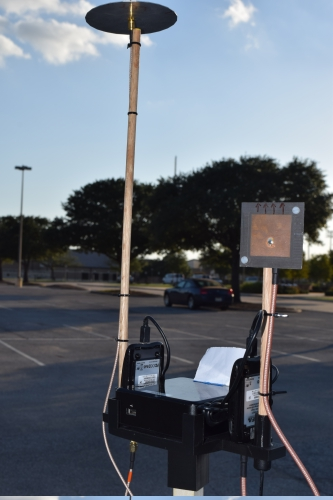
\includegraphics[scale=0.5]{Figures/DeviceSetup.jpg}
	\caption{This graph shows the monitoring device we use. }
	\label{figure: Device}
\end{figure}
The monitoring device we used during experiment is shown in Fig. \ref{figure: Device}.

\section{Wireless client}
In our experiment, the wireless clients are Android{\texttrademark} smartphones. All the wireless clients connect to a same local access point and send packets periodically which makes them detected by sniffing software. For the purpose of evaluate the performance of estimator, not only we need RSSI values, but we also need the ground truth (i.e. the location of the wireless clients). Thus we employ a custom app, which logs GPS coordinates and time. While conducting experiment, wireless clients periodically transmit the GPS information collected by app to a central server. MAC addresses and time stamps are then used to match locations to power vectors at the center server, yielding a data set for performance evaluation.

\section{Experimental Samples}
The experimental samples are divided into two categories, one is for monitoring devices with isotropic antennas, the other is for monitoring devices with directional antennas. Each category contains about 400 power and location vectors. Each power vector is in this form, $\underline{\mathbf{p}} = (\mathbf{p}_1, \ldots, \mathbf{p}_{4})$, where $\mathbf{p}_i$ is the power received by $i$ monitoring device. Since there are four monitoring devices, we have almost 3200 distinct points of RSSI. For conduct experimental trail as following. Firstly, generate the number of active clients inside $\r_{t}$ and number of active clients outside $\r_{o}$ according to two Poisson distribution with parameter $\lambda_{t}$ and $\lambda_[o]$ respectively. 
\begin{xalignat*}{2}
	\lambda_{\mathrm{t}}
	&= \alpha \frac{\lambda}{A_{\mathrm{t}}}
	&\lambda_{\mathrm{o}}
	&= (1 - \alpha) \frac{\lambda}{A_{\mathrm{o}}} .
\end{xalignat*}
Then $r_{t}$ entries are selected uniformly from clients in $A_{t}$, and $r_{o}$ entries are selected uniformly from clients in $A_{o}$. The two collections of entries are combined into a single vector $\underline{\mathbf{p}}$, which is the input to the estimator. At last, the estimates are evaluated through the ground truth.

\section{Channel Parameters}
Channel parameters $A$ and $B$ can vary depending on the wireless environment. This experiment is conducted on widely open parking lot. Fig.  offers a satellite image view of the experiment site.
The parameters are obtained by using least squares method mentioned in \ref{section:channel}. The parameters for the isotropic systems are $A = -41.68, B = -16.07$ and $\sigma_{s} = 7.91 dBm$. Similarly, the parameters for the systems with directional antennas are $A = -34.72, B = -17.11$ and $\sigma_{s} = 8.31 dBm$
\begin{figure}[]
	\centering
	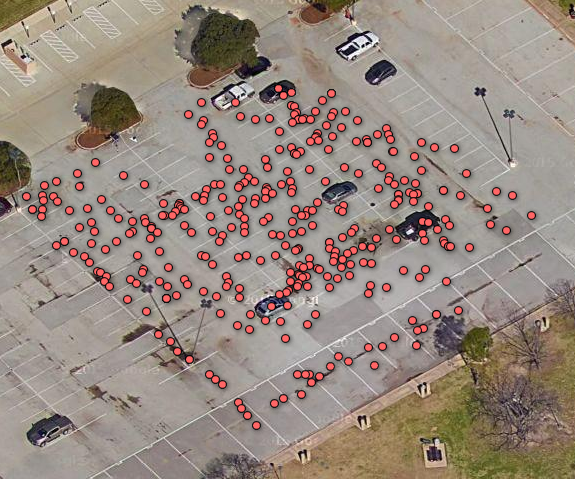
\includegraphics[scale=1]{Figures/Googlemap.png}
	\caption{This figure highlights the site used for the experiments and marks locations of experiment data. }
	\label{figure: Googlemap}
\end{figure}

\section{Experiment Results}
\subsection{Performance of Bayes Estimation}
Experimental curves under Bayes estimation scheme is shown in Fig. \ref{figure: bayesex}. The horizontal axis is the splitting parameter $\alpha$. The vertical axis is the BMSE. Each point is averaging over 10000 trails.
\begin{figure}[]
	\centering
	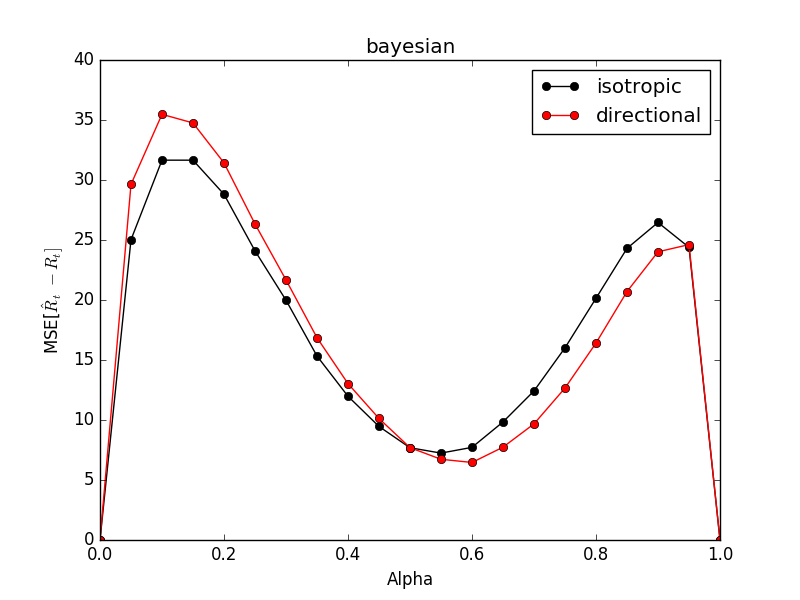
\includegraphics[scale=0.5]{Figures/bayesex.png}
	\caption{This figure depicts the experimental Bayesian mean squared error as function of Poisson splitting coefficient $\alpha$. Red line represents systems with directional antennas, whereas black line represent system with isotropic antennas. }
	\label{figure: bayesex}
\end{figure}
The confidence intervals of $|r_{t}-\hat{r_{t}}|$ corresponding to isotropic antennas and directional antennas are summarized in Table \ref{table:ConfidenceBayesex}.
\begin{table}[bht]
	\caption{Confidence interval of $|r_{t}-\hat{r_{t}}|$ for experimental Bayes scheme} \label{table:ConfidenceBayesex}
	\centerline{
		\begin{tabular}{|l|l|c|}
			\hline
			\multicolumn{1}{|c|}{\textbf{Antenna type}} &
			\multicolumn{1}{|c|}{\textbf{Confidence interval}} &
			\multicolumn{1}{|c|}{\textbf{Confidence level}} \\
			\hline
			Directional & $3.317535 \pm 0.010430$& 95\% \\
			\hline
			Isotropic & $3.331094 \pm 0.010274$ & 95\% \\
			\hline
		\end{tabular}}
	\end{table}
The approximation probability density functions corresponding to systems with directional antennas and isotropic antennas are shown in Fig. \ref{figure: bayesdirex} and Fig. \ref{figure: bayesomniex}.
\begin{figure}[]
	\centering
	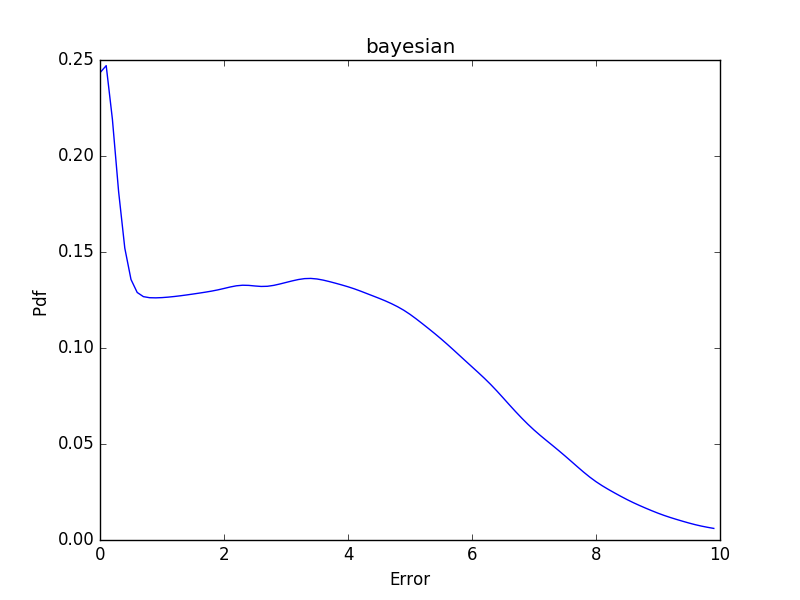
\includegraphics[scale=0.5]{Figures/bayesdirex.png}
	\caption{This graph shows the approximation probability density function of $|r_{t}-\hat{r_{t}}|$ corresponding to system equipped with directional antennas under scheme of \ref{section:BayesEstimation}. }
	\label{figure: bayesdirex}
\end{figure}
\begin{figure}[]
	\centering
	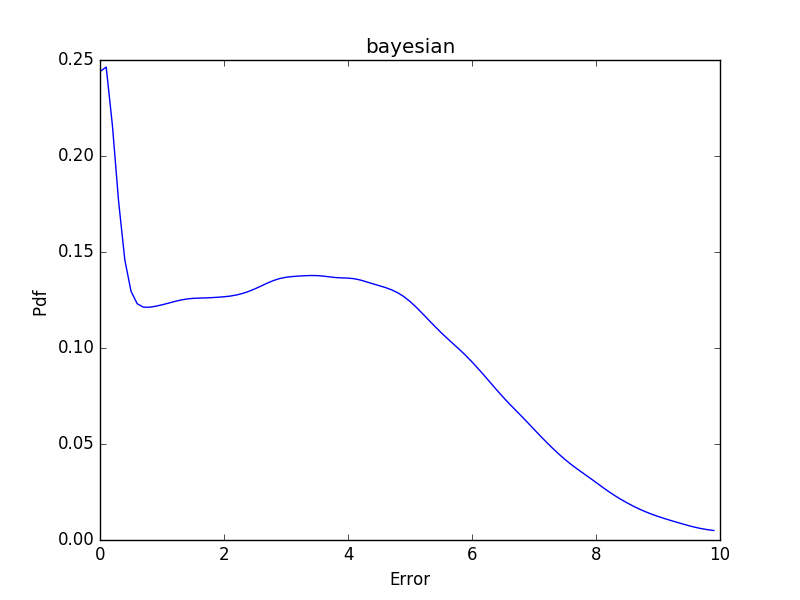
\includegraphics[scale=0.5]{Figures/bayesomniex.png}
	\caption{This graph shows the approximation probability density function of $|r_{t}-\hat{r_{t}}|$ corresponding to system equipped with isotropic antennas under scheme of \ref{section:BayesEstimation}. }
	\label{figure: bayesomniex}
\end{figure}
In this case using directional antennas does not bring an obvious benefit. The BMSE of systems with directional antennas and that with isotropic antennas are very close. As well as the confidence intervals and the absolute error distribution. This phenomena maybe caused by the inaccuracy of GPS information. Some small location errors may bring large errors, especially for the case when using directional antennas. 
\subsection{Performance of Maximum Estimation}
Experimental curves under Bayes estimation scheme is shown in Fig. \ref{figure: maxRTex}. The horizontal axis is the splitting parameter $\alpha$. The vertical axis is the BMSE. Each point is averaging over 10000 trails.
\begin{figure}[]
	\centering
	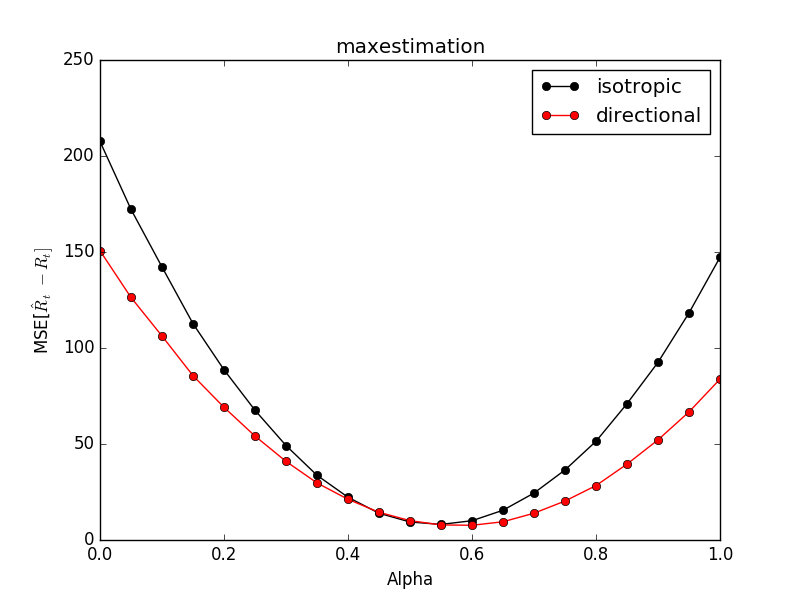
\includegraphics[scale=0.5]{Figures/maxRTex.png}
	\caption{This figure depicts the experimental Bayesian mean squared error as function of Poisson splitting coefficient $\alpha$. Red line represents systems with directional antennas, whereas black line represent system with isotropic antennas. }
	\label{figure: maxRTex}
\end{figure}
The confidence intervals of $|r_{t}-\hat{r_{t}}|$ corresponding to isotropic antennas and directional antennas are summarized in Table \ref{table:Confidencemaxex}.
\begin{table}[bht]
	\caption{Confidence interval of $|r_{t}-\hat{r_{t}}|$ for experimental Maximum estimation scheme} \label{table:Confidencemaxex}
	\centerline{
		\begin{tabular}{|l|l|c|}
			\hline
			\multicolumn{1}{|c|}{\textbf{Antenna type}} &
			\multicolumn{1}{|c|}{\textbf{Confidence interval}}&
			\multicolumn{1}{|c|}{\textbf{Confidence level}} \\
			\hline
			Directional & $5.881027 \pm 0.016484$ &95\% \\
			\hline
			Isotropic & $7.144900 \pm 0.019182$ &95\% \\
			\hline
		\end{tabular}}
	\end{table}
	The approximation probability density functions corresponding to systems with directional antennas and isotropic antennas are shown in Fig. \ref{figure: maxdirex} and Fig. \ref{figure: maxomniex}.
	\begin{figure}[]
		\centering
		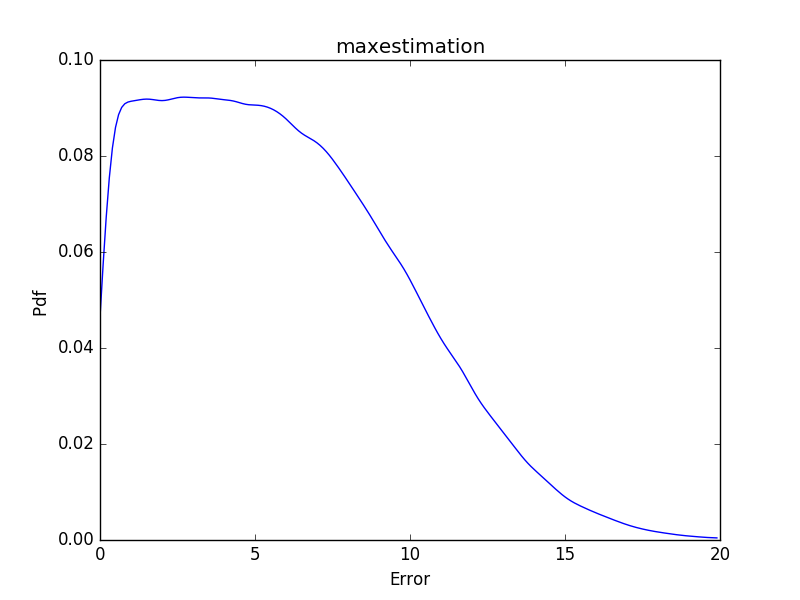
\includegraphics[scale=0.5]{Figures/maxdirex.png}
		\caption{This graph shows the approximation probability density function of $|r_{t}-\hat{r_{t}}|$ corresponding to system equipped with directional antennas under scheme of \ref{section:Maxestimation}. }
		\label{figure: maxdirex}
	\end{figure}
	\begin{figure}[]
		\centering
		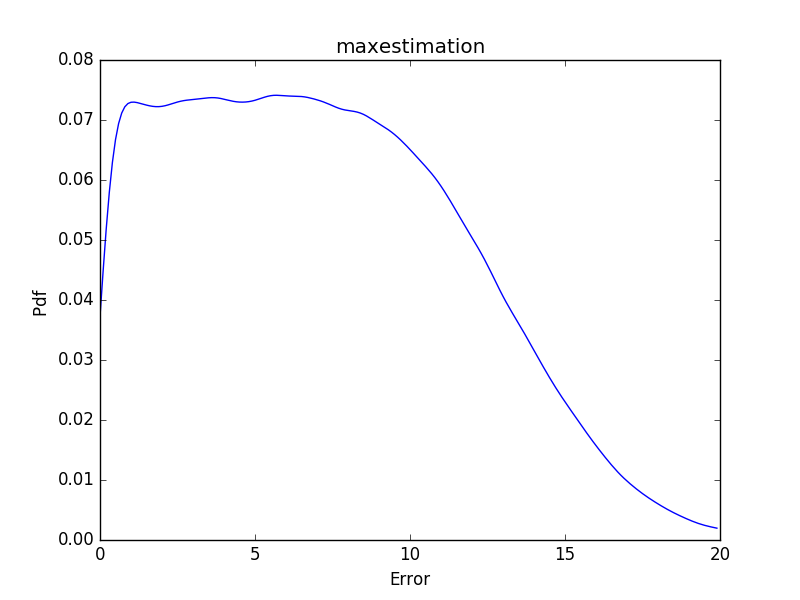
\includegraphics[scale=0.5]{Figures/maxomniex.png}
		\caption{This graph shows the approximation probability density function of $|r_{t}-\hat{r_{t}}|$ corresponding to system equipped with isotropic antennas under scheme of \ref{section:Maxestimation}. }
		\label{figure: maxomniex}
	\end{figure}
In this case, systems with directional antennas better, which means systems equipped with direcional antennas are more discrimination.